\chapter{Limit Setting and Results}

\section{Introduction}

Once the event selection and background estimation procedure have been defined
and the data has been collected one needs to determine the limit on the cross
section of a possible SUSY signal (according to a specific model) or, if a 
discovery has been made, the significance of that discovery. \\

In the present case no discovery has been made so a limit on the cross section
must be found. There are various statistical procedures for doing this and no 
consensus on the best method. If all methods give similar results, then it does
not matter which method is used. \\

A likelihood function must be defined. The likelihood is the probability of 
observing the data given a model. This encompasses the statistical uncertainties
and the background model as well as the systematic uncertainties associated
with the detector (e.g. luminosity measurement and jet energy scale uncertainty)
which affect the number of signal events expected. \\

Parameters in the likelihood should include the parameter of interest on which 
we wish to set a limit -- the cross section in this case -- in addition to
other unknowns associated with systematic uncertainties. \\

The goal is to find a confidence interval for the parameter of interest based
on the likelihood. This tells us an upper limit on the cross section of a
 possible SUSY signal at a given confidence level. \\

Three methods are used here for limit setting:
\begin{itemize}
\item Profile Likelihood using Wilks Theorem to find the confidence interval.
\item Feldman Cousins Method: using Neyman Construction to get the confidence 
interval with the Profile Likelihood as a test statistic.
\item CLs with MC toys using the Profile Likelihood.
\end{itemize}

\section{Likelihood Function}

Let: 
\begin{itemize}
\item $b$ = Estimated number of background events;
\item $s$ = Number of expected signal events according to a specific SUSY model;
\item $n$ = Number of events observed.
\end{itemize}

Considering only the statistical error on the expected number of events, which 
follows a Poisson distribution, the likelihood for the background only 
hypothesis is given by Equation \ref{eq:Poisson_Likelihood_BackgroundOnly}.

\begin{equation}
L_{b} = p(n|b) = \frac{b^{n}e^{-b}}{n!} 
\label{eq:Poisson_Likelihood_BackgroundOnly}
\end{equation}

And for the signal plus background hypothesis the likelihood is given by Equation
\ref{eq:Poisson_Likelihood_SignalPlusBackground}.

\begin{equation}
L_{s+b} = p(n|s+b) = \frac{(s+b)^{n}e^{-(s+b)}}{n!} 
\label{eq:Poisson_Likelihood_SignalPlusBackground}
\end{equation}

Using Equation \ref{eq:Number_of_signal_events} for the number of signal events, 
the likelihood for the signal plus background hypothesis can now be written as 
Equation \ref{eq:SignalPlusBackground_Rewritten}.

\begin{equation}
L_{s+b} = \frac{(\epsilon \sigma L + b)^{n} e^{-(\epsilon \sigma L + b)}}{n!} 
\label{eq:SignalPlusBackground_Rewritten}
\end{equation}

\section{Systematic Uncertainties}

Consider M sources of systematic uncertainty: $\sigma_{j}$, j = 1..M. Systematic
uncertainties can be introduced to the likelihood as nuisance parameters 
$\theta_{j}$ upon which $b_{i}$ and $s_{i}$ depend. Gaussian terms are added to 
the likelihood to constrain their values. For example if the integrated 
luminosity was measured to be $1.1 \unit{fb^{-1}}$ with an error of 4\unit{\%}, a Gaussian term 
with mean 1100 and sigma 44 would be added to the likelihood. Thus the central
value of the luminosity is allowed to fluctuate constrained by the Gaussian.
Equation \ref{eq:Full_Likelihood} shows the full likelihood function, including 
nuisance parameters. 

\begin{equation}
L_{s+b} = \prod_{i=1}^{N}
\frac{\left(\epsilon_{i} \cdot \left(\intlumi\right) \cdot \sigma+b_{i}\right)^{n_{i}}e^{-\left(\epsilon_{i} \cdot \left(\intlumi\right) \cdot \sigma+b_{i}\right)}}{n_{i}!} 
\cdot \prod_{j=1}^{M} \frac{1}{\sqrt{2\pi}\sigma_{j}}e^{-\frac{1}{2}\left(\frac{\theta_{j} - \mu_{j}}{\sigma_{j}}\right)^{2}} 
\label{eq:Full_Likelihood}
\end{equation}

\section{Test Statistic}

A confidence interval is calculated based on a test statistic. This can be the 
likelihood for the signal + background hypothesis. However this can be misleading
if the background hypothesis doesn't fit either. A more common approach is to 
use the likelihood ratio (Equation \ref{eq:Likelihood_Ratio}), where 
$\boldsymbol\theta$ is the vector of parameters and $\hat{\boldsymbol\theta}$
is the vector of parameter values which maximises the likelihood. 

\begin{equation}
-2\log\Lambda_{profile} = -2\log\frac{L_{s+b}(\boldsymbol\theta)}{L_{b}(\hat{\boldsymbol\theta})}
\label{eq:Likelihood_Ratio}
\end{equation}

For ease of calculation the negative log likelihood is used instead of the likelihood.
Both the likelihood and the negative log likelihood  must have an optimum at the same 
value whatever the form of the likelihood function since the logarithm is a monotonic 
function.

\section{Confidence Intervals}

\subsection{Wilks Theorem}

Wilks Theorem states that the negative log profile likelihood ratio is 
asymptotically distributed as a $\chi^{2}$ with N degrees of freedom, where N is
the number of parameters of interest. 

\subsection{Neyman Construction}

Consider a pdf $f\left(x;\theta\right)$ where $\theta$ is the unknown parameter 
we are trying to estimate: the cross section in our case. We wish to construct a
confidence interval for $\theta$. \\

Step through possible values of $\theta$. For each value of $\theta$ find a range 
$\left(x_{1},x_{2}\right)$ such that a fraction $1 - \alpha$ of the $x$ 
distribution lies within the range, see Equation \ref{eq:Neyman_Interval}. 
$1 - \alpha$ is the confidence level.

\begin{equation}
\int_{x_{1}}^{x_{2}} f\left(x;\theta\right) = 1 - \alpha
\label{eq:Neyman_Interval}
\end{equation} 

Figure \ref{fig:Confidence_Belt} shows the ranges $\left(x_{1},x_{2}\right)$ as
horizontal line segments on the $\left(x,\theta\right)$ plane for each possible 
value of $\theta$. \\

\begin{figure}
\begin{center}
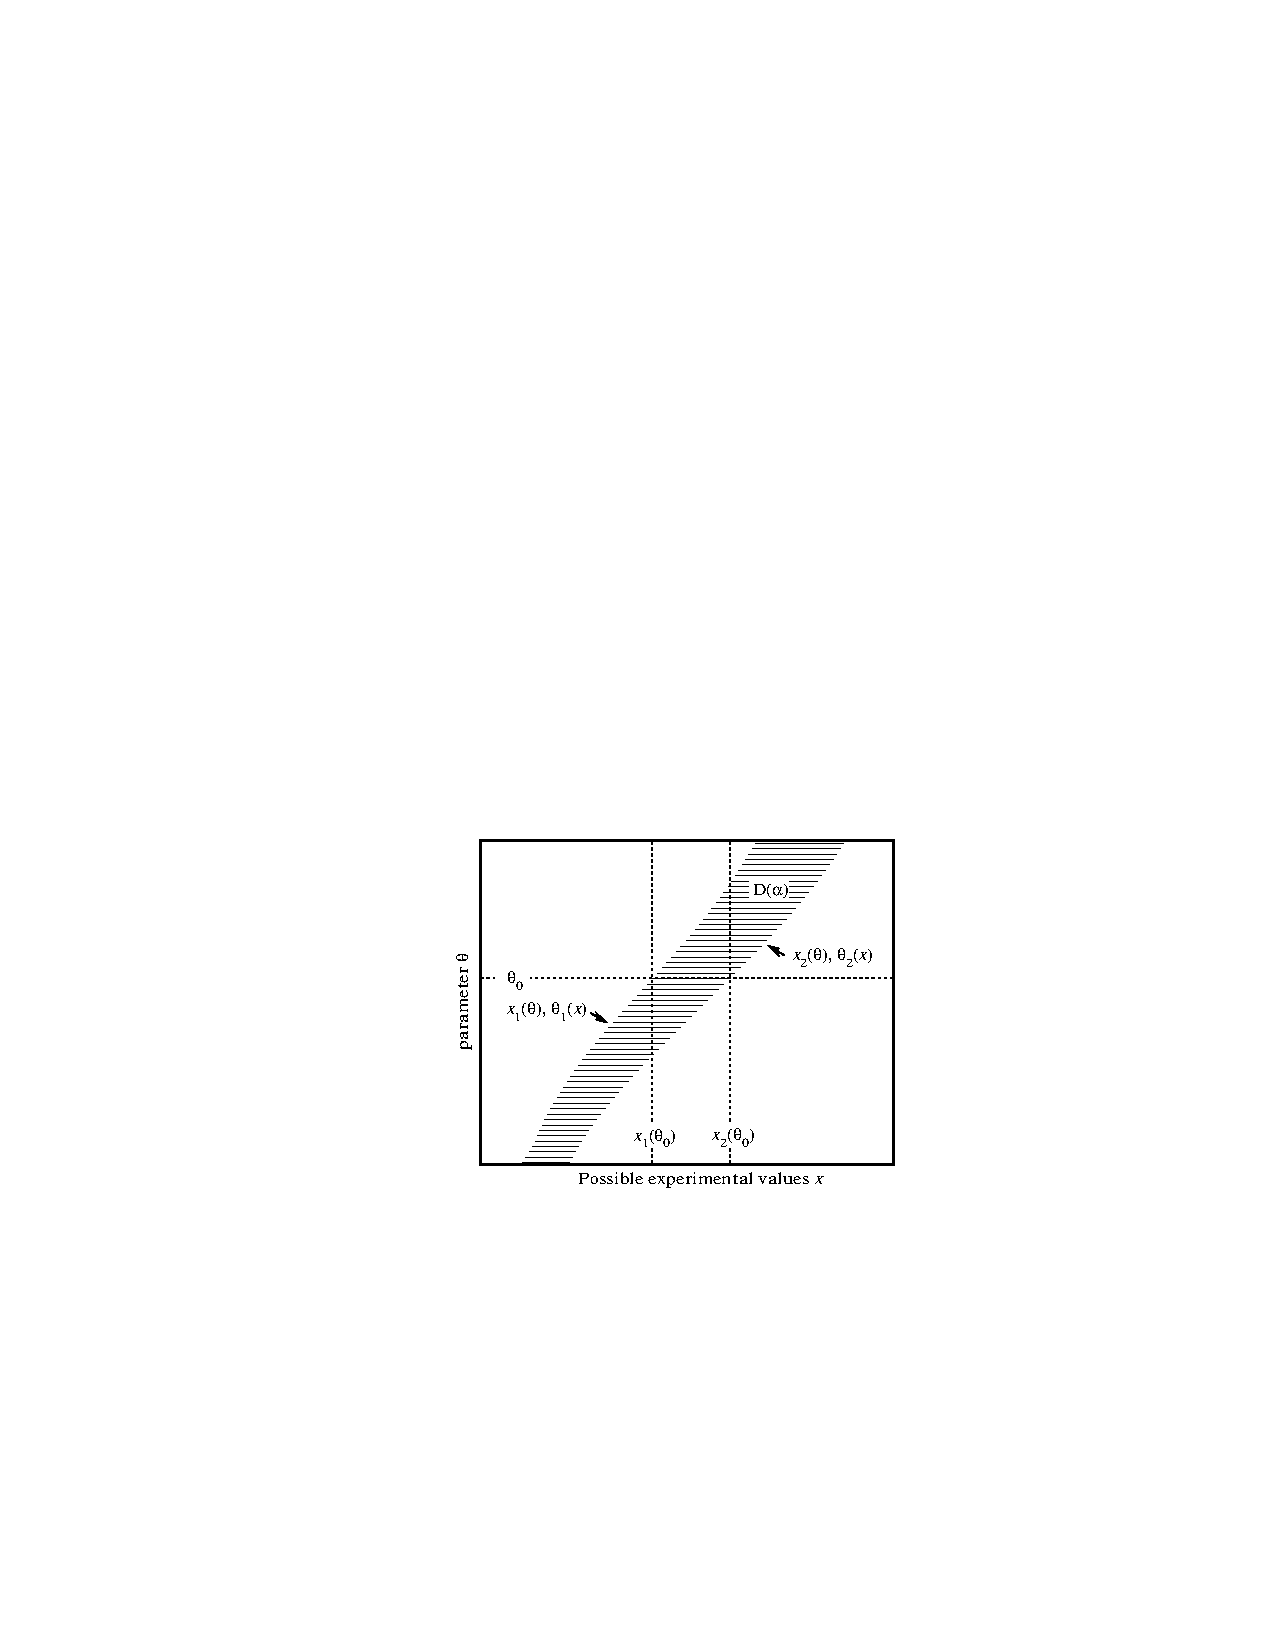
\includegraphics[width=0.8\textwidth]{Confidence_Belt.pdf}
\caption{The ranges $\left(x_{1},x_{2}\right)$ as horizontal lines in the 
$\left(x,\theta\right)$ plane for each possible value of $\theta$. A
confidence belt is marked out the vertical height of which gives the
confidence interval for each possible measurement value.}
\label{fig:Confidence_Belt}
\end{center}
\end{figure}

Upon measurement of $x$ as having value $x_{0}$ we draw a vertical line on the 
$\left(x,\theta\right)$ plane (Figure \ref{fig:Confidence_Belt}) at $x = x_{0}$.
Under the Neyman Construction the confidence interval for $\theta$ is defined by
the values of $\theta$ where the vertical line intersects the horizontal ranges 
$\left(x_{1},x_{2}\right)$. \\

The Neyman Construction is not a unique procedure: it does not specify how the 
ranges $\left(x_{1},x_{2}\right)$ which contain $1 - \alpha$ of the pdf should
be found. A rule for ordering the $x$ values (test statistic) is required. \\

In the Feldman Cousins method the ordering principle is the likelihood ratio -- 
motivated by the Neyman-Pearson lemma. When nuisance parameters are involved the
profile likelihood ratio is the natural generalisation.

\subsection{CLs: MC toys with hypothesis testing}


\section{Expected and Observed Limit}

An expected limit without looking at the data can be calculated. Pseudo data is
generated using the background model. An expected limit is calculated using any
of the above methods using the pseudo data as if it were data. \\

Many sets of pseudo data are generated and a limit on the cross section of a 
possible SUSY signal is calculated for each. An expected limit can be drawn on 
the SUSY parameter space by linking those parameter points for which the cross 
section can be excluded at 95\% confidence level in half of the pseudo 
experiments -- the median of excluded cross section across all pseudo 
experiments. $1 \sigma$ and $2 \sigma$ bands, lines linking the parameter points
where the cross section is excluded for 67\% and 95\% of the pseudo experiments 
respectively, are also drawn.
